\documentclass{article}
\usepackage{graphicx} % Required for inserting images
\usepackage{placeins}


\title{Research Idea Matthijs Muis}
\author{Matthijs Muis}
\date{April 2023}


\usepackage{multicol}
\usepackage[utf8]{inputenc}     % for éô
\usepackage[english]{babel}     % for proper word breaking at line ends
\usepackage[a4paper, left=1in, right=1in, top=1in, bottom=1in]{geometry}
                                % for page size and margin settings
\usepackage{amsmath,amssymb}    % for better equations
\usepackage{amsthm}             % for better theorem styles
\usepackage{mathtools}          % for greek math symbol formatting
\usepackage{enumitem}           % for control of 'enumerate' numbering
\usepackage{listings}           % for control of 'itemize' spacing
\usepackage{todonotes}          % for clear TODO notes
\usepackage{hyperref}           % page numbers and '\ref's become clickable

%% SET TITLE PAGE VALUES HERE 
\def\thesistitle{Improving data efficiency and alleviating the problem of constrained exploration in RL HVAC control using Model-Predictive Controllers}
\def\thesisauthorfirst{Matthijs Muis}


%% FOR PDF METADATA
\title{\thesistitle}
\author{\thesisauthorfirst}
\date{May 19, 2023}


%% THEOREM STYLES
\newtheorem{theorem}{Theorem}[section]
\newtheorem{corollary}{Corollary}[theorem]
\newtheorem{lemma}[theorem]{Lemma}
\newtheorem{proposition}[theorem]{Proposition}

\theoremstyle{definition}
\newtheorem{definition}[theorem]{Definition}

\theoremstyle{remark}
\newtheorem*{remark}{Remark}


%% MATH OPERATORS
\DeclareMathOperator{\supersine}{supersin}
\DeclareMathOperator{\supercosine}{supercos}


%% SHORTCUT NOTATIONS
\newcommand{\mar}{\mathcal{M}}
\newcommand{\stat}{\mathcal{X}}
\newcommand{\act}{\mathcal{A}}
\newcommand{\prob}{\mathcal{P}}

\newcommand{\N}{\mathbb{N}}
\newcommand{\R}{\mathbb{R}}

%%%%%%%%%%%%%%%%%%%%%%%

\begin{document}
\maketitle
\tableofcontents

\newpage

\section{Outline of the problem}
\subsection{Topic}
In 2016, Deepmind reported that through application of its artificial intelligence technologies, it had been able to reduce the power consumption of Google's data centers by 40 \% \cite{evans_gao_2016}. Given the state-of-the-art efficiency of Google's data centers at the time, this meant a major breakthrough in the theory of control systems. The algorithm used reinforcement learning (RL) to learn the complex dynamics of the data center's cooling system. Another algorithm was developed in a more general datacenter setting \cite{gamble_gao_2018}. Later, Deepmind refocused on heating, ventilation and air-conditioning (HVAC) control systems and developed a deep reinforcement learning (DRL) controller named BCOOLER \cite{luo2022controlling}. 

Traditional HVAC control systems typically rely on simple feedback loop heuristics, called the \textit{sequence of operations} (SOO). These heuristics are sometimes based on predictions from an additional physical model for heat transport in the building, in which case we speak of model-predictive control (MPC) \cite{Schwenzer_Ay_Bergs_Abel_2021}. Heuristic models have simple feedback loop policies that miss many physical dynamics and do not plan at all \cite{killian2016ten, Schwenzer_Ay_Bergs_Abel_2021}. MPC uses a deterministic physical model of the building to optimize its actions, and while this approach is able to succesfully plan over finite horizons \cite{privara2011modeling}, it picks up no more complex dynamics than those envisioned by the designers \cite{luo2022controlling}. What is more, these models are ignorant of important non-physical influences such as building occupancy \cite{killian2016ten}. 

In contrast, an RL algorithm in principle requires no assumptions on the internal physical model of the data center: it learns optimal control actions directly from its interaction with the system. This was observed when Google's data center algorithm took ``advantage of winter conditions and produce colder than normal water, which reduces the energy required for cooling within the data centre'' \cite{gamble_gao_2018}. The potential of the RL framework has been noticed: Yu et al. report a surge of interest of the application of, in particular, Deep RL to autonomous HVAC control \cite{Yuetal}.

\subsection{Knowledge gap}
\subsubsection{Data efficiency through Model Based Reinforcement Learning}
There are however still many barriers to take before the RL approach to HVAC controllers can become a mainstream framework. \cite{luo2022controlling} mentions as future work that ``Data efficiency could be improved by adding additional domain specific inductive biases to the model, such as the physical topology of the equipment in the facility, or the constraints and invariances of the sensor measurements given by first principle physics''. Current approaches to reinforcement learned HVAC control are model-free, which means that the agent has no physical model of the environment it interacts with: it only contains a regression model to predict action-values from potential action-state pairs, which it optimizes over a generated set of actions. There are three limitations to this ``tabula rasa'' approach that a complementary physical model might be able to address.

First, generating sufficient actions to maintain good exploration is difficult due to the high dimensionality of the action space in HVAC applications: the BCOOLER algorithm had to generate 100k actions to maintain good exploration (see sec. 8.6, \cite{luo2022controlling}). But the paper also mentions that with only 4 values per dimension, it would have needed to check over 10M actions per time-step.

Second, training of a model-free agent is difficult to do in a live environment, due to the invasiveness of training sessions for building occupants and equipment. Most of the research mentioned in \cite{Yuetal} train and evaluate RL agents all in a simulated environment. Deepmind's papers are quite unique in this aspect. \cite{evans_gao_2016, gamble_gao_2018, luo2022controlling} approach the issue in two steps: first, pre-train the agents on offline data (\textit{Offline Reinforcement Learning}) collected from the existing SOO, and then fine-tune in an live session by \textit{Constrained Reinforcement Learning} (CRL) under safety constraints. A lot of work went into specifying hard (non-violable) and soft (penalized) constraints, which turned out to be rather difficult: ``[...] we found it very hard to elicit specific penalty values for a soft constraint formulation, and impossible to guarantee that a hard constraint formulation as a function of future observations will be satisfied.'' \cite{luo2022controlling}.

The third problem of model-free RL is that it is difficult to know whether a trained agent can generalize to other facilities. The spectacular efficiency gains reported by Deepmind in \cite{gamble_gao_2018, luo2022controlling, evans_gao_2016} were all achieved in with model-free agents, i.e. agents that directly estimate the action-value function of the decision problem (for terminology, see \ref{theory:RL}). The action-value estimation is typically an opaque regresssion function, i.e. a deep neural network. Because it behaves like a black box, we cannot predict how the agent will act in other environments. The application of one learned agent is narrowed to the facility, while training the agent was difficult. Moreover, there is no contribution to the current body of scientific knowledge when the agent fails to improve power efficiency.

General constrained reinforcement learning is an active area of research \cite{agarwal2020optimistic}, as is offline reinforcement learning, \cite{levine2020offline}. But little research has explored the potential of leveraging domain-specific knowledge in a Model Based RL agent (such as described in \cite{Seita_2019}), at least not in HVAC control of office buildings. 

However, deterministic optimal control theory has already developed a rich body of knowledge on Model-Predictive Control (MPC) \cite{Schwenzer_Ay_Bergs_Abel_2021} However, the model does not predict its future cost, meaning that there is little learning from the environment.

As we will see in the theoretical framework, the theories of RL and MPC show great similarity. We propose research into a framework for an RL agent that uses a Model Predictive Controller to generate actions that satisfy soft constraints. The aim is to alleviate the problem of dimensionality of the action space, to leverage the MPC to satisfy constraints, while keeping the constraints soft in order to elicit safe exploration. Summarizing, we want to make RL-based HVAC control easier. 

This is an excellent topic of further investigation, because even if the first experiments are not quite successful, it will still lay the foundation for the unification of the theory of MPC with RL. We can already rely on a rich body of theory involving model-based reinforcement learning, e.g. from the sources mentioned in \cite{Seita_2019}, so this is not at all an infeasible goal. Another motivation, namely the potential environmental benefits, will be further detailed under \ref{motivation}.

\subsection{Problem formulation}
\subsubsection{Overview}
We give an overview of the structure of the proposed MPC-RL agent, which we call $A$. It is shown in figure \ref{fig:hybrid}. The agent consists of:
\begin{enumerate}
    \item Inputs for observable variables $x_t$, collected at discrete time-steps $t$ from sensors in various spaces of the facility, e.g. temperature, air humidity. 
    \item Inputs for setpoints or reference variables $s_t$, that are set by building occupants: these are temperatures specified on e.g. thermostats.
    \item Outputs for control variables, also called action variables, which turn on/off cooling or heating equipment and provide setpoints to them.
    \item A Model-Predictive Controller $B$ that takes the physical state variables $x'_t$ in $x_t$ and computes a cost-minimizing control strategy consisting of a finite trajectory of actions $a_t, a_{t+1}, ... a_{t+T}$. The \textit{cost} function of the action trajectory $(a_{ji})_{j=t}^{j=t+T}$, which further dependends on the current setpoint $s_t$ future trajectories $(x'_j)_{j=t}^{j=t+T}$ of states, denoted $J((a_{j})_{j=t}^{j=t+T}| (x'_{ji})_{j=t}^{j=t+T},s_t$, is defined as the expected energy usage per calculated load (for HVAC terminology, see \ref{theory:HVAC}) with added quadratic penalty terms for the distances between setpoints and the required future state variables. The MPC can calculate optimal trajectories that minimize $J$ on the fly, using numerical methods. This numerical method we adapt to instead give a \textit{set} of many cost-minimizing trajectories $\{(a_{ji})_{j=t}^{j=t+T}\}_{i\in I}$.  This is our solution to constrained exploration: rather than filtering a large set of randomly generated actions on hard constraints like in \cite{luo2022controlling}, we use the direct optimization capabilities of the MPC to generate already regularized actions. 
    \item A regression function, which is in RL theory known as the action-value predictor or the \textit{critic}, $C$ for which we take a convolutional neural network (CNN) architecture similar to BCOOLER \cite{luo2022controlling}. The critic takes the first action of the trajectory $a_{ti}$ generated by $B$ and the current state $x_t$, including non-physical data that $B$ does not take into account, such as time-of-day and day-of-year (to make long-term strategies that take into account day/night and seasonal influences) and returns an estimation of the optimal action value $Q^*(x,a)$, $\hat Q(x_t, a_t)$. The action-value is defined as the long-term reward of the 
    \item An actor that simply takes the actions $\{a_{ti}\}_{i\in I}$ and picks the action that the critic evaluated as having the highest $\hat Q(x_t,a_t)$. This is the RL-part of the agent that will learn to predict optimal action-values by interaction with the environment.
\end{enumerate}

\begin{figure}
    \centering
    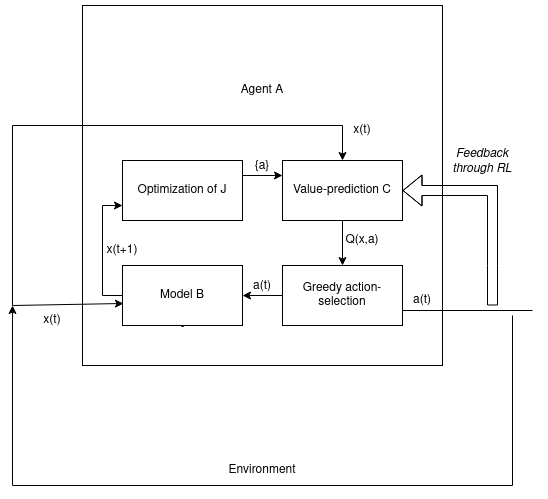
\includegraphics[width=3in]{thediagram.png}
    \caption{Diagram showing the outline of the hybrid MPC/RL model $A$}
    \label{fig:hybrid}
\end{figure}

The idea is that the MPC perceives the controlled environment as modelled by its own predictive physical model. The RL agent perceives the environment as within the framework of RL, that is, as a Markov Decision Process (MDP). It sees a richer set of non-physical  variables, which cannot be modeled within a simple MPC. This allows it to develop richer strategies. Both models both have different definitions for their cost (reward): the MPC selects action trajectories that minimize $J$, defined as the average energy used per load plus additional penalty terms to regularize actions. The RL agent is not required to regularize anything, since it can only consider actions that are regular by definition of $J$: its immediate reward is simply the negative of used energy, while it tries to optimize for the expected long-term reward $Q$. Details on terminology can be found under \ref{theory:HVAC}, \ref{theory:RL}. The models are discussed further under \ref{Method:modelA}, \ref{Method:modelling:B}.

The RL agent will interact with the environment, using stochastic gradient descent to iteratively improve the parameters of $C$ to predict the optimal action-value $Q^*(x_t,a_t)$. For the details we refer to \ref{theory:RL}. The MPC will not learn its parameters but plays an important role in providing constraint-satisfying actions for the RL part of the agent. On the other hand, the RL part of the agent complements the MPC by adding more finer tactics and strategies to the HVAC control that are too difficult to envision or implement in the MPC.

After designing a set of architectures for the predictive model, we pre-train the critic using RL in an environment that can be simulated using the same predictive model $B$ uses. When the critic shows sufficient convergence, we train it for another three months in the live facility and then evaluate it: we  compare its strategy's average energy consumption and benchmark against an existing SOO, both at a live facility and in a simulated environment. To account for confounding factors, i.e. situations that increase the energy consumption of any controller (we should not compare the energy consumption of a controller on a wintry day to that of a controller on a temperate day), we take inspiration from \cite{luo2022controlling} and compare mean energy consumption of both models only for time points that have a similar outside \textit{wet bulb temperature} (see \ref{theory:HVAC}) and load (see \ref{theory:HVAC}). For the quantitative details we refer to \ref{Method:DatAn:confounders}. 

The trial should take a year to collect data for all seasonal weather types. The safety of building occupants is assured through a hierarchical approach, where the original sequence of operations (SOO, i.e. controller) takes over if the penalizing terms become too large.




\FloatBarrier


\subsubsection{Research question}

The main research question can be summarized as: \\
\textit{How will the energy efficiency of the HVAC installation of a medium-sized building with t change compared to an existing SOO with the above proposed method, and how will the parameters of critic $C$ change during the RL session? }

The scale of the building at which the system is employed is important to mention, as it determines the dimensionality of the action space.

Subquestions include:
\begin{enumerate}
    \item Does the trained critic prefer actions that are considerably different from the unique optimal action computed by the MPC?
    \item Which model architecture for the critic has the fastest convergence of parameters during simulated training?
    \item Which model architecture for the critic picks the most optimal actions?
    \item Which statistical technique should be used to quantitatively compare the performance of this model with the original SOO?
\end{enumerate}

These subquestions can help guide picking the right critic to continue with during online testing.

\subsubsection{Symmetry of outcomes}
Although the most interesting scenario would be to see the model outperform than the original SOO, the scenario of no significant improvement would not be useless. Note that underperformance is a logical impossibility as the proposed controller is ensured to have at least the degrees of freedom as the original SOO. 

The second scenario would still mean benefit to the current body of knowledgde of both MPC, RL and HVAC control, because the framework remains, which can always be reused with a new predictive model substituted for $B$. In future research, $B$ might even be replaced by a machine-learned model itself. The framework will be written in an object oriented fashion and can be integrated with new modules easily.

As a second argument for the utility of the product, we point to the learned critic $C$. Its parameters are more interpretable than in a model-free agent such as BCOOLER \cite{luo2022controlling}, because we can clearly distinguish which part of the agent does the prediction and which part the decision making. So if $A$ fails to perform better, the trace of its parameters can at least be analyzed meaningfully. Perhaps $C$ did not converge, or overfit during training, being swung up and down by the changing of day to night or seasons which the original MPC was insensitive to. Either way, the trace of the parameters of $C$ will contribute to the current body of knowledge by providing future attention points to scientists and engineers who want to further with the proposed framework.

\subsection{Motivation} \label{motivation}
\paragraph{Door to generic, mainstream optimization of HVAC control}
Unlike existing research into RL control for HVAC, the proposed framework does not intend to discard the predictive model that is central to MPC. This makes the model data-efficient and non-invasive: it utilizes online RL only to tune the parameters It additionally requires considerably less thinking about the constraints and suitable constrained-RL methods. This makes the usage of the framework generic and simple. 

The framework we create is generalizable to generic combinations of critics and MPCs, and thus to different facilities that already employ MPC. At the same time, it is easy to pre-train offline and relatively noninvasive to then train online, making the approach accessible for mainstream building tenants. The difficulties of constraint formulation is avoided and that of the dimensionality of the action space is mitigated considerably. This should make the framework scalable. If succesful, the approach to training RL algorithms studied in this research could open the door to a generic, simplified method for partial on-line training of RL HVAC controllers in applications. 

The potential of these adaptive controllers has been shown in the aforementioned research, but seems to be limited to companies who can afford this approach by their scale, such as Google with its datacenters that have a large expenditure on cooling. This makes the main-stream application of these controllers still far away if the training process cannot be simplified dramatically.

\FloatBarrier
\paragraph{Environmental impact}



\begin{figure}
    \centering
    \includegraphics[width=3in]{Emissions-by-sector-–-pie-charts.png}
    \caption{Energy use in commercial buildings accounts for 6.6\% of global GHG emissions. Source: \cite{owidco2andgreenhousegasemissions}}
    \label{fig:ghg emissions}
\end{figure}

HVAC systems make up a large portion of the energy consumption (EC) and greenhouse gas (GHG) emission of commercial buildings, and estimatedly 98\% of EC and GHG emission is from the lifetime of operational energy and not from the manufacturing and production energy \cite{co2emissionsfromhvacequipment,COLE1998335,SUZUKI199833,lifecycleenergyanalysis}. In 2016, energy use in commercial buildings made up for 6.6\% of global GHG emissions \cite{owidco2andgreenhousegasemissions}, see figure \ref{fig:ghg emissions}. Space cooling in general accounts for 10\% of the global electricity demand \cite{futureofcooling}. Improvements such as reported in \cite{evans_gao_2016} would thus mean a great benefit to the environment, reducing global GHG emissions by $40\% \cdot 6.6\% \approx 2.6 \%$. 

But we repeat that the development of these algorithms needs to be simplified in order for them to become mainstream: research such as \cite{evans_gao_2016, luo2022controlling, gamble_gao_2018} is only reserved for companies who can apply their trained algorithms at a large scale and thus can afford the investment. The tabula rasa approach to RL comes with too many obstacles to be feasible for small-scaled facilities, which means that most commercial buildings will not see these being applied anytime soon.

A framework such as proposed here builds on years of experience of MPC theory to reduce the problem of action generation and avoid the problem of constraint formulation and satisfaction, which is a notable problem in model-free RL. The ``domain inductive biases'' added by the predictive model will allow for partially offline training combined with online finetuning. Even if the results are not positive at first, the novel approach and software framework that will be developed in the process can be used with different action-value-predictors or MPCs. 

The framework is not only flexible, but its training is easier, much less invasive compared to the completely model-free RL models, making it ideal to experiment on and learned from in future work. This wil certainly open the doors to improvements in energy efficiency. The framework is much more general and can be widely deployed when in the future, so it always holds the potential of having a great environmental impact in the future. It might even be possible to generalize to residential buildings, cutting into another 10.9\% of global greenhouse gas emissions \cite{owidco2andgreenhousegasemissions}.

\FloatBarrier

\paragraph{Model transparency and interpretation.}
As discussed above, the seperation of decision-making and prediction inside the agent makes it possible to assign some meaning to the parameters in critic $C$. This critic might also correct for, and point out, sensor miscalibrations in the existing installation that a conventional SOO would not be able to discover. This has been reported in prior research, see e.g. appendix B.2 of \cite{luo2022controlling}.

\section{Theoretical framework}

\subsection{HVAC control systems}\label{theory:HVAC}
We first introduce some useful terminology regarding space heating and cooling, which can be found in chap. 18 of \cite{ashraeHandbook}:

\paragraph{\textit{Load}:} this is the internal energy that needs to be removed from or added to the atmosphere in order to satisfy the current demand.

\paragraph{\textit{Wet-bulb temperature (WBT)}:} Traditionally, the temperature read by a thermometer covered in water-soaked cloth over which the air is passed. At 100\% air humidity, the WBT equals the temperature, otherwise it is lower than the actual air temperature. WBT is an accurate measure for how much cooling is necessary because it takes into account \textit{latent internal energy} contained in the water vapor in the air.

\paragraph{\textit{Capacity}} of an HVAC installation is the maximum load per unit time that the installation can remove from any space.

The energy-efficiency of an HVAC controller is measured as its average energy consumption. This energy consumption is not directly related to the load, but also depends on the outside wet-bulb temperature. As an example, by simply opening a vent on a cold day, a controller can easily remove a large load from a space at a minor energy consumption. This also shows how efficiency of a controller depends highly on the cooling strategy. We can also name more complex examples, such as energy saved by the correct use of a heat pump to store and reuse removed load.

\subsubsection{SOO types}
An HVAC installation is controlled by a rule-based control system called the \textit{sequence of operations} (SOO). This system can turn on pieces of equipment and can provide \textit{setpoints} to them. These setpoints are target values to be achieved on the individual equipment level \cite{luo2022controlling}. Achievement of the setpoint is thus delegated entirely to equipment, which usually accomplishes this through the aforementioned feedback-loop system. 

The controller can only see the achieved value and setpoint, and usually receives new measurements of these discrete time intervals. For large numbers of equipment, the total number of combinations of setpoints suffers from the curse of dimensionality \cite{luo2022controlling}, i.e. the action space gets very large. This makes it impossible to generate actions from the entire action space, and this might hamper the exploration of an RL agent.

\FloatBarrier
Several types of heuristics exist that the SOO can be based on:


\begin{figure}
    \centering
    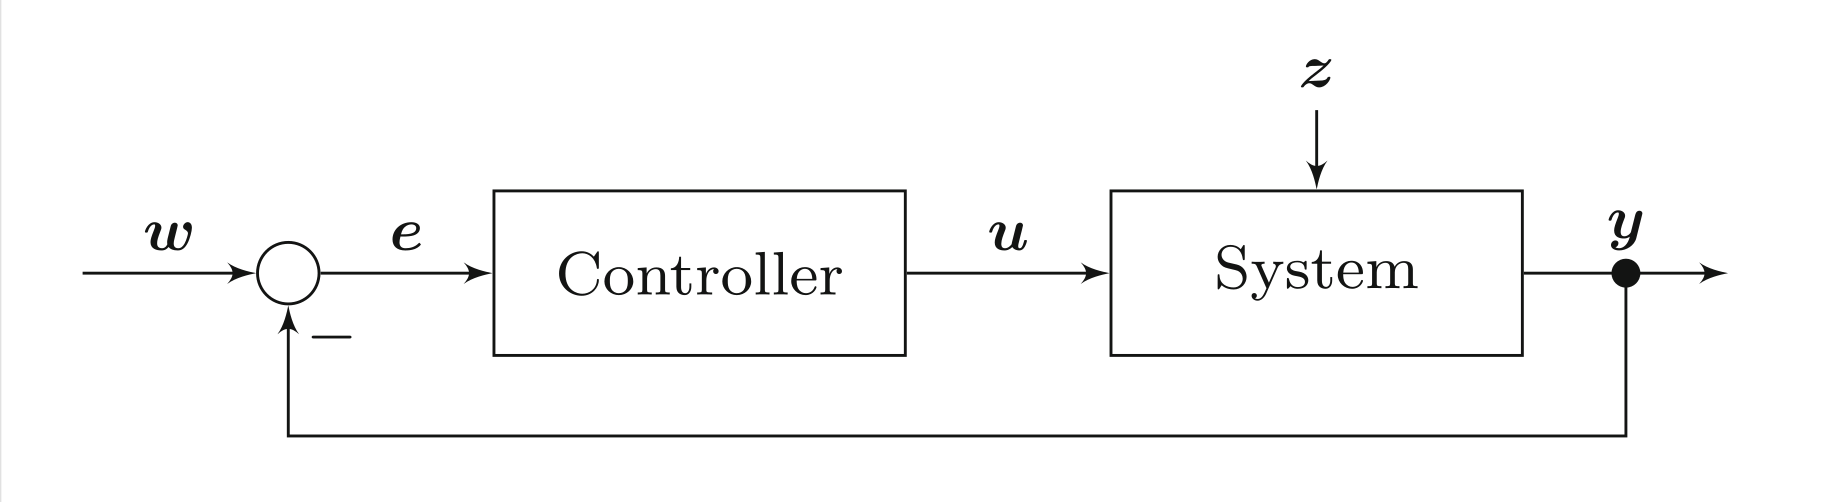
\includegraphics[width=3in]{feedbackloop.png}
    \caption{A simple feedback-loop controller, such as a PID controller. Source: \cite{Schwenzer_Ay_Bergs_Abel_2021}}
    \label{fig:simplefeedback}
\end{figure}


\paragraph{Direct feedback-loop}: The difference between the demanded control variable value and the actual control variable value determines the setpoint of the equipment \cite{Schwenzer_Ay_Bergs_Abel_2021}. An advanced example of this is the PID-controller (PID standing for Proportional, Differential, Integral). The heuristic here is very simple and does not allow for planning of the control actions over a longer period of time.



\begin{figure}
    \centering
    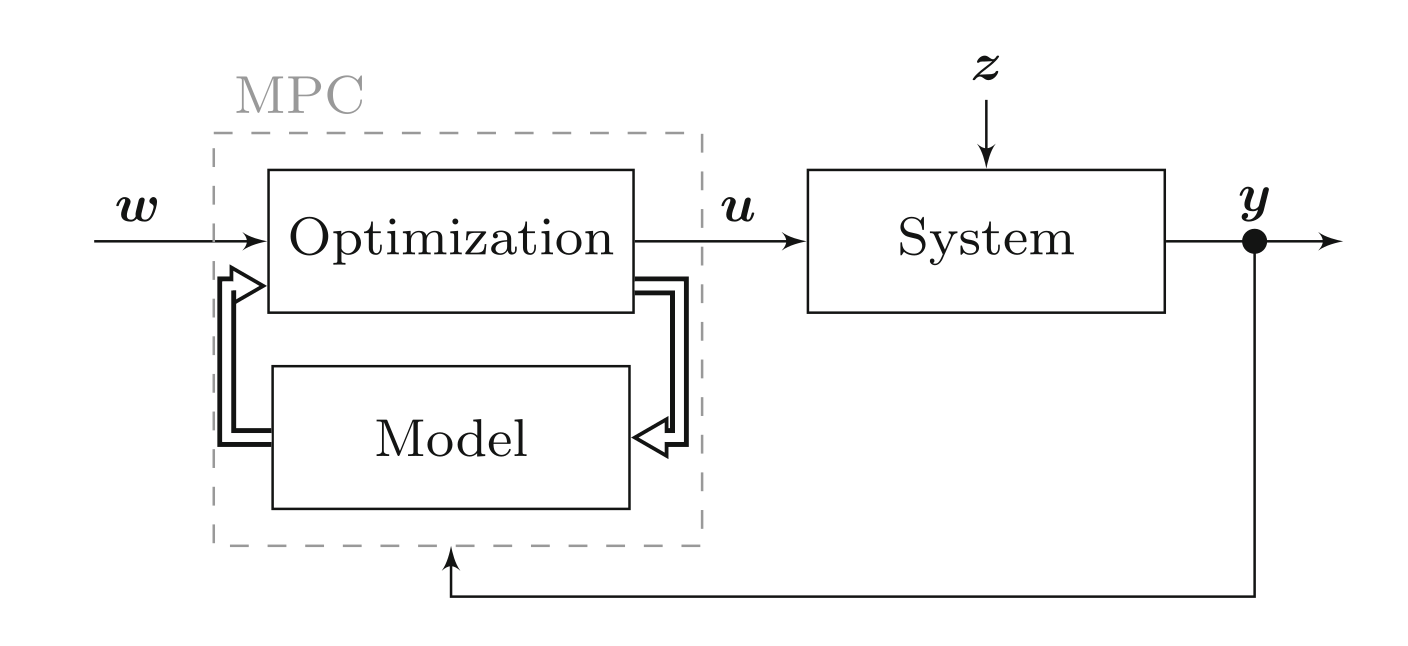
\includegraphics[width=3in]{mpc.png}
    \caption{An MPC controller. Source: \cite{Schwenzer_Ay_Bergs_Abel_2021}}
    \label{fig:mpc}
\end{figure}

\paragraph{MPC-based}
Our new RL agent will be built around an existing MPC controller. In MPC, the prediction of the future state of the system based on action and current state is given by a physical model. This physical model is given as an equation, i.e.:
\begin{equation}\label{equation}
    x_{t+1} = B(x_t,a_t)
\end{equation} 
Where $B$ is a function dependent of $x_t$ and $a_t$. 
The other part of the MPC framework consists of a \textit{cost function} $J$. $J$ is usually a sum that includes terms that penalize energy usage, as well as terms that penalize the deviation of the future state trajectory from the current setpoint. The negative of the cost function can be compared to the action-value function $Q$ from RL theory, described under \ref{theory:RL} and in \cite{suttonbarto2018, Szepesvari2010}. The important difference however is that there exists an explicit optimization algorithm that can calculate a trajectory of actions that minimizes the cost function $J$, i.e. to minimize the following formula:
\begin{equation}\label{opttt}
    \min_{(a_t)_{t=t_0}^{t=t_0+T}} \sum_{t=t_0}^{t_0+T}J(a, x_t, s_t)
\end{equation}


In order for this to be possible, the predictive model \ref{equation} has to be simple enough. It is usually linear; a well-known example of such a predictive model is the Kalman filter \cite{kalman1960contributions}.


We use different letters for the variables than conventional literature (e.g. \cite{Schwenzer_Ay_Bergs_Abel_2021}) to emphasize the relationship with RL, which is discussed below
Constraints can be added if necessary, although our approach will be to include them as penalty factors in $J$, see e.g. the function in \cite{privara2011modeling}. The difference is that in constrained optimization, the constraints are ``hard'', i.e. they bound the area in which the solution should be sought, while penalty factors make the constraints ``soft'': they can be violated if it ultimately optimizes \ref{opttt}. 

For an overview of MPC various models that implement the MPC framework and in particular their accompanying numerical optimization techniques that they employ, see \cite{QIN2003733}. For an introduction to the theory, we refer to \cite{rawlings2000tutorial}.


\FloatBarrier
\subsection{Reinforcement learning}\label{theory:RL}

Reinforcement learning (RL) studies machine learning in the framework of a Markov decision process (MDP)
We will simply focus on the terminology and notation here. A detailed exposition of MDPs, RL and 
algorithms can be found in \cite{suttonbarto2018} and \cite{Szepesvari2010}

\begin{definition} A Markov decision process (MDP)  $\mar$ is a triple $\mar = (\stat, \act, \prob)$
Where $\stat$ is a countable set, also called the \emph{state space}, $\act$ is a countable set of actions and $\prob: \stat \times \act \rightarrow (\stat \times \R \rightarrow [0,1])$, $\prob: (x,a) \mapsto \prob_{(x,a)}$ a \emph{probability kernel} that assigns to every pair in $(x,a) \in \stat \times \act$ a probability measure $\prob_{(x,a)}:\stat \times \R \rightarrow [0,1]$. We denote the stochastic variable distributed according to $\prob_{(x,a)}$ as $(X,R)$ and it is further assumed that $R$ is bounded almost surely.
\end{definition}
This is the definition given in \cite{Szepesvari2010}.
Note that the definition imposes countability on the state and action space, which makes it
easier to define general algorithms for these models.

The interpretation of $\mar$ is as follows: for each state $x\in\stat$ an \emph{agent} can choose any
action from $\act$ and this gives a probability distribution over pairs of $(x,r)$ where $x\in\stat$ 
is the next state of the system and
$r\in \R$ is the immediate \emph{reward} the agent receives. 

Many problems that involve sequential 
decisions can be modeled by an appropriate state-reward space. By the definition, the model
assumes that the distribution for next state-reward pairs will only depend on the current state and
action taken. This property is referred to as the \emph{Markov} property of the model. Often when modelling
problems as MDPs one simly assumes this property or defines the state space such that each
state $x\in \stat$ also keeps the appropriate details of the history of the process up to the current state.

The goal one hopes to achieve is to find a strategy or policy $\pi : \stat \rightarrow \act$ such that if in
every state $x\in\stat$ the agent picks policy $\pi(x)$, the maximum achievable expected long-term reward is achieved. Generalizing further, the policy should sometimes be defined as a probability measure $\pi_x:\act \rightarrow [0,1]$ if the agent has to act unpredictably in order to play optimally. This is the case in a suitable
MDP model of the
game of rock, paper, scissors, for example. In HVAC controller systems, it is usually preferred that at least the controller itself behaves deterministically.

The goal of maximizing the expected reward can be formalized as follows:

\begin{definition} Given an MDP $\mar=(\stat,\act,\prob)$ and a (deterministic) policy $\pi$, the MRP $\mathcal{R}^pi$ is a tuple $(\stat, \prob^\pi)$ where $\prob^\pi:\stat\rightarrow \stat\times\R$ is the probability kernel given by $x\mapsto \prob_{(x,\pi(x))}$.
\end{definition}

\begin{definition} Fix a $\gamma \in ]0,1[$. The \emph{value} $V:\stat \rightarrow \R$ of an MRP $\mathcal{R}$ is given as:
\begin{equation}
V(x) = \mathbb{E}\left[ \sum_{t=0}^\infty \gamma^tR_{t+1} \ \vert \ X_0  = x\right]
\end{equation}
Where the sequences $(X_t)_{t\in\N}$, $(R_t)_{t\in\N}$ denote the stochastic sequences that are induced by $P$, where $X_t$ denotes the state at time $t\in\N$. These are determined entirely by the conditional distributions
\begin{align*}
    (X_t,R_t)|(X_j=x_j,R_j=r_j)_{j=0,..t-1}  &\sim (X_t,R_t)|(X_{t-1}=x_{t-1}) \\ (X_t,R_t)|(X_t=x_t) &\sim \prob_x
\end{align*}
\end{definition}

We can extend this definition to MDPs:

\begin{definition}
Fix a $\gamma \in ]0,1[$. The \emph{value} $V^\pi:\stat \rightarrow \R$ of the MDP $\mathcal{M}$ is given by
the value function $V$ of the MRP $\mathcal{R}^\pi$
\end{definition}

The final useful definitions involving policies and values:

\begin{definition}
Fix a $\gamma \in ]0,1[$. The \emph{action-value} $Q^\pi:\stat \times \act \rightarrow \R$ of the MDP $\mathcal{M}$ is given as:
\begin{equation}
Q^\pi(x,a) = \mathbb{E}\left[ V^\pi (X_1) + R_1 \ \vert \ (X_1,R_1) \sim \prob_{(x,a)}\right]
\end{equation}
Again, here we let $((X_t,A_t,R_{t+1})_{t\in \mathbb{N}}$ denote the stochastic process.
\end{definition}

Solving an MDP means: to find a policy $\pi$ that maximizes $V^\pi$ uniformly over $\stat$. The value of such a policy is $\pi^*$ is written as $V^*$ and called the \textit{optimal value function}. It satisfies, by definition:
\begin{equation}
  V^*(x) = \max_{\pi\in\Pi} V^\pi(x)  
\end{equation}
Where $\Pi$ denotes the set of all stochastic stationary policies \cite{Szepesvari2010}. We see that this equation is only sensible when the policy $\pi^*_x$ that maximizes the right hand side is the same for all states $x$, because this is what, by definition, \textit{uniform} maximization over $\stat$ requires. 

Analogously to $V^*$, we can define the \textit{optimal action-value function} $Q^*$ of $(x,a)\in \stat \times \act$ as the optimal value plus expected immediate reward given state $x$ and action $a$.

\subsubsection{Additional notation}

\paragraph{Transition probability} The probability measure $\prob$ gives rise to a state transition probability $\prob : \stat \times \act \times \stat \rightarrow [0,1]$ which assigns to every triple $(x,a,y)$ the probability that the system transitions to state $y$ given action $a$ and current state $x$.

\paragraph{Expected reward (1)} For every pair $(x,a)\in \stat \times \act$ we can define ${r(x,a) := \mathbb{E}[R_{t+1} \ | \ X_t = x, A_t = a]}$. Note that this is well defined due to time-homogeneity of the process.

\paragraph{Expected reward (2)} For every pair $x\in \stat$ we can define ${r(x) := \mathbb{E}[R_{t+1} \ | \ X_t = x]}$. Again, this is well defined due to time-homogeneity of the process.

\subsection{Reinforcement learning algorithms}
\subsubsection{Optimality as a fixed point}

Uniform maximization is possible in the more well-behaved class of MDPs when we allow for the aforementioned stochastic policy type \cite{Szepesvari2010}. Let $Y^X$ denote the set of all functions $X\rightarrow Y$. Also, let $r(x,a)$ When dealing with not all too exotic MDPs  we are concerned with deterministic policies, we see that in general $Q^\pi$ and $\pi$ need to satisfy the \textit{Bellman Equation} \cite{suttonbarto2018, Szepesvari2010}:
\begin{align}
    T^\pi Q^\pi &= Q^\pi \\
    T^*Q^* &= Q^*
\end{align}

Where we define $T^\pi, T^*$ as $\R^{\stat\times \act} \rightarrow \R^{\stat\times \act}$: 
\begin{align}
    (T^\pi Q)(x,a) &:= r(x,a) + \gamma \sum_{y\in \stat} \prob(x,a,y)Q(y,\pi(y)), & (x,a)\in \stat \times \act \\
    (T^* Q)(x,a) &:= r(x,a) + \gamma \sum_{y\in \stat} \prob(x,a,y)\sup_{a'\in \act}Q(y,\pi(y)), & (x,a)\in \stat \times \act
\end{align}

Further, we note that it is enough to know $Q^*$ to deduce $\pi^*$, as:
\begin{align}
    \pi^*(x) &= \text{arg}\max_{a\in \mathcal{A}} Q^* (x,a), &\forall x \in \mathcal{X}
\end{align}

\subsubsection{On-Policy iteration}
The problem here is that the terms on both sides depend on $\pi^*$, which needs to be found. The method of policy iteration approaches the problem of solving this equation for $\pi^*$ as follows:

\begin{enumerate}
    \item \textit{Action-value estimation:} Simulate of the MRP given by the MDP followed under $\pi_k$. This is followed by an appropriate (statistical) estimation $\hat Q^\pi_{k+1}$ of the function $Q^\pi$ for a current policy $\pi_k$.
    
    \item \textit{Policy update:} Find the new $\hat\pi_{k+1}$ that is optimal with respect to the newly estimated $\hat Q^\pi_k$.
\end{enumerate}

The intuitive idea is that every iteration $k$ $\hat Q^\pi_{k}$ will be more accurate, meaning that the policy $\hat\pi_k$ can be estimated closer to the optimal policy $\pi^*$, which in turn implies that $\hat Q^\pi_{k+1}$ will resemble the action value for optimal continuation of the strategy, i.e. the function $Q^*$, more closely. One might point here to the circularity of this argument. Yet, various theorems from the field show that many RL algorithms that at a high level based on this process, indeed converge on some fixed points for $Q$ and $\pi$, which in the case of the right choice of parametrization (i.e. model architecture) for $\hat Q$ and $\hat\pi$ would indeed approximate the optimal action-value and optimal policy. For a brief overview of convergence criteria, see \cite{leemondu}.

When the action and/or state space is high-dimensional, it is often infeasible to keep an estimation of $Q(x,a)$ and $\pi(x)$ for every pair $(x,a) \in \stat\times\act$, the so-called \textit{tabular approach} \cite{suttonbarto2018, Szepesvari2010}. The alternative approach is to use a parametric model for $Q^*$ and estimate the parameters instead. This is the so-called \textit{value-function approximation}. The simplest approach is to only parametrize the value function $Q^\pi$ through a parameter $\theta$, and then to iteratively:
\begin{enumerate}
    \item \textit{Action-value estimation:} Simulate of the MRP given by the MDP followed under $\pi_k$. $\pi_k$ is defined as the policy that simply picks an action $a$ that optimizes the current estimate $\hat Q(x_t,a)$. 
    
    \item \textit{Learn from experience:} Based on the reward that was estimated and the reward that was actually received, an appropriate (statistical) estimation of the parameter $\theta$ is done to improve the estimate $\hat Q^\pi_{k+1}$ of the function $Q^\pi$ for the current policy $\pi_k$.
    
    \item \textit{Policy update:} $\pi_{k+1}$ is defined as the policy that simply picks the action $a$ that optimizes the current estimate $\hat Q(x_t,a)$. with respect to the newly estimated $\hat Q^\pi_k$.
\end{enumerate}

There are many variants on both action-value estimation and policy-update methods, of which a detailed exposition can be found in \cite{suttonbarto2018, Szepesvari2010}. The algorithm proposed in our research will be discussed under \ref{Method:RLAlg}.



\section{Method}
The method can be separated into a design phase and an experimentation phase. First, the design stage is outlined. Then, the experimentation stage is discussed. \ref{Method:setup} discusses the general setting of the controller. Finally, a time plan for both phases is given under \ref{time plan}.

\subsection{Design stage}
\subsubsection{Setting and resources}\label{Method:setup}
We will train the agent in the Mercator II building of Radboud University Nijmegen. This is a multi-tenant office building, housing companies with a close connection to the Faculty of Science of this university \cite{MercatorSciencePark_2023}. This choice has several reasons:

\begin{enumerate}
    \item The researcher is a student of Radboud University and expects the building tenant to be open for student innovation in the realm of energy-saving. 
    
    \item The design of the building had energy-efficiency in mind from the inception of the plan, see e.g. the project description of the architect, \cite{PauldeRuiter_2023}. Because of this, we expect smaller noise in the efficiency of control systems employed in this environment. This is beneficial when comparing performances of the RL agent to the original SOO.
    
    First, it means that random confounders (i.e. open windows, doors) if they arise, do not lead to such high variance in performance variables as in buildings not designed with these influences in mind. 
    This is beneficial because mitigating the influence of confounders, means our measurements of the performance difference between the extension and the original become more accurate. 
    
    Second, a consciously energy-efficient design might mean a higher density of sensors and actuators, which will allow us to collect more relevant data and give the model a finer control of the environment.

    Third, we hope that the energy-efficient design also comes with an extensive SOO for the HVAC control of the building.
    
    \item The building houses offices only, in contrast to e.g. the Huygens building on the same campus, which has added demand in cooling and heating from its many laboratories.
\end{enumerate}

The building has a bruto floor area of 7.000 m$^2$, and has the uniform shape of an elongated cube. Designed by Paul de Ruiter architects, its (HVAC) equipment is due to Boonstoppel Engineering and Deerns \cite{PauldeRuiter_2023}. In order to make a model of the building together with its different space blocks, sensors, actuators and thermostats, we will need to consult these three parties. \footnote{From correspondence with Deerns, we collect that the original design was by Boonstoppel, which was later acquired by Deerns. As it appears, most people involved in the project are now retired. Deerns spokesperson adviced to consult facility of the university itself to acquire the design plans.} We also need to discuss with them the heuristics underlying the original SOO, and ask about the availability of historical data collected by this SOO.

Further, if not present we need to install sensors on the outside of the walls of the building. This is because we want to collect data from the environment of the building in order to better model the heat flow. This is also done because the weather (wet-bulb) temperature of the is a confounder when comparing performances of $A$ against $B$ (see \ref{Method:DatAn:confounders}

\paragraph{SOO requirements} we do require the SOO to have an internal MPC model, as this will provide the basis for model $B$. If the provided SOO does not satisfy this requirement, we must design a feasible MPC. This will be a linear MPC that we import from prior research in MPC-based office cooling performed at Hollandsch Huys \cite{hollands}. The new parameters of this imported SOO MPC controller are estimated for the setting of Mercator II. We will benchmark the final model against power consumption data of the original SOO of the facility.

\subsubsection{Observed features}\label{Method:FeatureSel}

The system will then be modeled as follows:
First, the internal space of the building is partitioned in segments that correspond with spaces that have restricted air flow between them. The goal of this is that sensors, actuators and demand-setters (i.e. thermostats that are set by building occupants) from space blocks that are adjacent should be modeled as \textit{local receptive fields} in the CNNs that form the architecture of model $B$. The reason for this approach are detailed under \ref{Method:modelling:B}. 

We also require every demand-setter to be paired with a sensor, since we need to calculate the difference between the demanded temperature and the achieved temperature. This is typically already the case as every piece of equipment typically relies on a feedback-control loop to achieve and maintain its setpoint. Finally, we require a time-of-day and day-of-week input for the models, which can be provided by a timing function in the computer system where the models are trained.

We expect the available sensors to measure the variable in which demands are expressed, namely air temperature, but also other variables such as humidity and possibly air pressure, to infer the WBT as a more accurate measure of load. These measurements are typically collected at discrete, regular time intervals (see \ref{theory:HVAC} which provides a natural discretization of the timeline for the MDP. We should collect what quantities are measured and in what units. We expect the original control system to already provide us with a central interface to collect this sensory data.

\subsubsection{Simulation environment}
In order to train $A$, we will make a model of the Mercator II building, if not provided by the engineers of Boonstoppel. This can be done in one of the many software packages available to this end, such as the open-source software package HVACSIM+ developed by the NIST \cite{Galler_2021}. Since the tool is quite complex and the designer has probably already done work on it, we definitely need to consult the engineering team for Mercator II on their modelling work.

\subsubsection{MDP formulation} \label{Method:MDP}
\paragraph{State space}
The states $x_t\in \mathcal{X}$ are defined as $N+4$-tuples of the form ${x_t = ((L^n\textbf{T}_t)_{n=0,1,..N}, (L^n\textbf{D}_t)_{n=0,1,..N}, \textbf{S}_t, \tau_t)}$. This representation contains:
\begin{enumerate}
    \item $\textbf{S}_t \in \mathbb{R}^d$, a vector of $d$ demanded setpoints from thermostats in the building. These are all demands expressed as a temperature.
    \item All temperature sensor data $\textbf{T}_t \in \mathbb{R}^d$ received from $d$ sensors that are paired to the $d$ thermostats in the building. These pairs are selected based upon distance between the setter and sensor. Of both $\textbf(S)$ and $\textbf{T}$, the last $n$ measurement instances preceding $t$, along with a vector of setpoints $\textit{S}_t$ demanded from the thermostats. Here, we use the convenient notation $L$ for the \textit{lag operator} $LT_t := T_{t-1}$. $N$ is a to be determined hyperparameter \footnote{With this, we assume that the process is Markovian with respect to this state space, which might approximately hold if we include enough lagged sensor measurements of previous time intervals. The choice of the hyperparameter $N$ leads to a trade-off between data and dimensionality, which has to be delved into deeper during the design. One can separate the observations from the state-space, which gives rise to a so-called Partially Observed MDP (POMDP). However, this is rarely done in practice since it complicates the model quite a lot. This proposal uses ``observation'' and ``state'' interchangeably}
    \item Sensory data $\textbf{D}_t \in \mathbb{R}^p$, which is the vector into which all other sensor measurements are collected. These include temperature data from sensors that could not be paired to a thermostat, but also sensors for humidity. Like $\mathbf{T}$, the state is determined by both current measurements as lagged measurements $L^n\mathbf{D}_t$.
    \item The time-of-day and day-of-week timings collected in $\tau_t\in \{0,1,..24\}\times \{1,2,..7\}$
\end{enumerate}
We will also use the predictive model to do a load calculation. The load and WBT are important in the analysis part of the benchmark stage.

\paragraph{Action space}\label{MDP:actions}
As discussed under \ref{theory:HVAC}, the control system can only influence the HVAC system by turning on and of pieces of equipment (actuators) in certain places and providing a setpoint for them. The way of achieving the setpoint is delegated to the local equipments, which usually uses a feedback loop for this \footnote{This usually implies that actuators for heating are paired with a sensor for heat in the vicinity, and the same goes for AC actuators and humidity and temperature sensors.}. The action space $\act$ thus consists of the cartesian product of consinuous ranges of setpoints, all ranges are paired with a binary variable that takes values in $\{$on, off$\}$. The exact ranges of setpoints along with minor alterations to the aforementioned structure depend on what we find when investigating the equipment.

\paragraph{Rewards and constraints} \label{constraints}
The reward function is not directly trivial in this setting. The problem is that the agent has three objectives:
\begin{enumerate}
    \item Minimize the difference between the demanded WBT and the actual WBT,
    \item Minimize the total power consumption of the equipment per load,
    \item Control the equipment in a sustainable and careful way.
\end{enumerate}
An agent that prioritizes the first criterium will probably skyrocket Mercator's energy bill, while an agent that prioritizes the second will leave poor office workers in freezingly cold rooms on a wintry day. We follow the implementation of criteria that is presented in most literature: 
\begin{enumerate}
    \item \textit{The reward} is the negative of the total power consumption per estimated load of the HVAC equipment, $\frac{-P_t}{l(x_t)}$ (which must be maximized). Load calculation $l(x_t)$ is done by the simulation software based on first-principle physical formulas.
    \item  The deviation between thermostat setpoint and actual temperature $\mathbf{T}_{t+1}-\mathbf{S}_{t+1}$ of the next state should always be bounded, leading to a constraint on the future state distribution \cite{gamble_gao_2018, evans_gao_2016, luo2022controlling}. 
    \item Additional direct constraints on the actions $a_t$ should prevent unresponsible usage of the equipment, e.g. continuously turning on/off the AC. This second constraint type requires keeping track of past actions. But these past actions do not have to be part of the state representation, because the constraints are not part of the MDP, but part of the constraint optimization programme $J$. 
\end{enumerate}
    The novelty that the action-selection based on cost-minimization of $J$ can bring, is that constraints do not have to be implemented as constraints on the RL agent, but can also be added as constraints \textit{or} as \textit{penalty terms} to the optimization criterium. Since we can simulate and thus try many models, we can empirically test which configuration yields fastest convergence and optimal efficiency.


\subsubsection{General modelling considerations}
We want the architecture of $B$ to take into account the topology of the building: this is done through a convolutional neural networks (CNN). In the first hidden layer of a convolutional neural network a neuron is connected to only a small subset of adjacent neurons in the input layer, in contrast to a regular neural network that has connections between all neurons of consecutive layers. Such groups of neurons in the CNN are called \textit{local receptive fields}, and their aim is to represent the topology or geometry of the input being analyzed: in our case, it does not make much sense to connect two sensor inputs from completely different parts of the building to the same hidden neuron, since the measurements from these sensors have no interesting relationship. However, it would be useful to investigate local relationships between adjacent rooms. 


\subsubsection{Model architecture of model A} \label{Method:modelA}
A picks an action $a_t = \pi(x_t)$ from the action set (described under \ref{theory:HVAC}) generated by the discussed constraint optimization in the MPC model $B$  and model-free action-value prediction $C$. This has been visualized in figure \ref{fig:hybrid}. The expected reward $Q(x,a)$ from RL theory and the cost function $J$ from MPC theory are the same object in this context, but within the MPC it is treated as a to be optimized function and then in the action-value approximator it is treated as a nondeterministic variable that needs to be predicted. 

\subsubsection{Model architecture of model B}\label{Method:modelling:B}
$B$ predicts the future state of the system, and to decide which of the proposed actions $a'$ optimizes the future state of the system, hence $B$ maps $(x,a') \mapsto x'$ where $x'$ is the likely future state. It is imported as an existing MPC that has been designed and tested by experts in that field. We need to expand the constraint optimizer of the model in order to generate a discretized set of actions in the neighbourhood of the action that follows from optimizing $J$. Proper ways of discretizing the action space in the vicinity of an optimum can be copied from section 8.6 in \cite{luo2022controlling}.

$B$ can only see the state variables that are used in the physical model. Contrast this to $C$, which also receives data on occupancy rate, time-of-day and day-of-year, day-of-week to develop richer strategies.
\subsubsection{Model architecture of model C}
Model $C$ is a CNN with convolutions with local receptive fields for adjacent rooms and space blocks. It is inspired on BCOOLERs architecture which was proven quite efficient \cite{luo2022controlling}. The exact geometry of the network is difficult to specify yet, as this is determined by the available input sensors. We will also try various depths of the network during the simulated training and pick the architecture with best convergence properties and performance in the simulation. 

We do not regard rooms that are located above each other on subsequent levels to be adjacent, as the bulk mass of the floor between them transfers heat negligibly slowly. We regard outdoor sensors on the walls of the building as adjacent to the rooms directly behind that wall on that floor. This is because the sun can significantly heat the outside wall of the building which leads to a higher demand for cooling in that sector of the building.

\subsubsection{Supervised and Reinforcement learning algorithm} \label{Method:RLAlg}
\paragraph{Action-value estimation}
This is done for $C$ during the RL training, in order to improve prediction by $B$ and to improve action-value estimation by $C$, and this can be achieved through backpropagation \cite{suttonbarto2018, Szepesvari2010} in the supervised phase.

In the reinforcement learning phase, this is done based on stochastic gradient descent. The parameter update is an appropriate scaling of the local gradient of the \textit{observed} loss function $\hat l$ that computes the difference between $\hat Q(x,a)$ and $r(x,a)$ for every state and taken action. Updating the parameters in the direction of this gradient will lead to a better estimate of the parameter $\theta$ in $B$.

\paragraph{Policy update}

This is done implicitly through updates of the action-value estimator $C$, by selecting the action $a$ that optimizes $\hat Q^*(x,a)$, which is the estimate provided by $C$. 

\subsection{Experiment}
\subsubsection{Data collection} \label{Method:DatC}
This section describes the data collection in the experiment that is necessary to evaluate the performance of the RL model against the original SOO. We collect and store:

\begin{enumerate}
\item The time series data of states, ${x_t = ((L^n\textbf{T}_t)_{n=0,1,..N}, (L^n\textbf{D}_t)_{n=0,1,..N}, \textbf{S}_t, \tau_t)}$.
\item The time series of historical data by the original model, called $\mathcal{H}$. This time series might have data of different dimensions due to missing sensors. For how this could be handled in the analysis we refer to \ref{Method:DatAn}.
\item The time series data of taken actions, both during final deployment of the $A$, and from the original SOO, which are certainly of the same dimensionality as we have not altered the actuator topology of the HVAC system.
\item The time series data of predicted reward/power consumption $(\hat Q(x_t,a_t))_{t\in\N}$, computed for both $A$ during deployment as for the original SOO. This together the time series of actual reward/power consumption for both $A$ and original SOO.
\item The time series data of load calculations and outside WBT (the WBT is actually already included in the state variables).
\end{enumerate}

The live testing will take place over the course of one year. This is to get a diverse sample from all different seasonal weather types. We need to check that the agent generalizes well. The agent needs to be active continuously in order to generate reliable data, since alternating it with the original SOO will result in the agent itself making biased predictions about future states and rewards (since it would estimate these as if it has full control, while in reality it only has control half of the time).

\subsubsection{Measurement}\label{Method:DatAn}
This concerns the measurement of dependent experimental variables, not the collection of sensory data to be used by the controller (which is discussed above). The succes of the training method can be quantified through the measurement of difference $\Delta P$ in the long-time average energy-to-load \textit{efficiency} (see \ref{theory:HVAC})of the trained controller $A$ compared to the MPC controller preceding it, in \textit{similar states} of the system (i.e. similar weather conditions, current temperatures and demand setpoints).

These measurements are directly logged by the installation on-site and can be logged in the simulation environment HVACSIM+ \cite{Galler_2021}.

\subsection{Data Analysis}
The aim is to compare performance of the original SOO and $A$. This can be done in both live trials as in a simulated environment. The second option is considerably cheaper and less involved while the first option provides the richer dynamics of true physical reality. We settle on a hybrid approach, using simulation to gather most of the data and using shorter trials to validate the precision of simulation.

We can rely on a large body of knowledge regarding building simulation software, this being the principal mode of model evaluation in most research on HVAC RL, as e.g. mentioned in \cite{Yuetal}. We also expect a building simulation model to be prepared for the training of model $B$ and $A$. We can log the efficiency directly from these simulations. Then, we simulate the original SOO in the same software model and compare the results for comparable loads.

\subsubsection{Confounders} \label{Method:DatAn:confounders}
When benchmarking model $A$ against $C$, we should be careful to account for confounding factors.
\begin{enumerate}
    \item The power consumption not only depends on the model, but more importantly on the load and the weather, i.e. power consumption for heating is certainly higher when it is freezing outside, compared to mild weather. This means that power consumption data from both models should only be compared for states that have similar weather types. The problem that follows, is how to measure the similarity of weather types in terms of expected power consumption.
    \item Another confounding factor noted in \cite{luo2022controlling} is the building occupancy level, which significantly influences the demand for heating , ventilation or AC.
    \item The final confounder we note is the influence on HVAC demand due to difficult-to-measure effects such as open doors and/or windows.
\end{enumerate}

\subsubsection{Solution: Partitioning of the sample}
These factors can be summarized as follows: they all increase or decrease the load for HVAC in some way, thereby influencing the power usage in the next state(s), without the model itself being able to do anything about it. Solutions to these confounders have been studied. The best method we found was given by \cite{luo2022controlling}: to compare the RL controller 
to the original SOO, the average power consumptions for similar loads and WBTs were compared for statistically significant differences. It produced the following very informative figure:

\begin{figure}
    \centering
    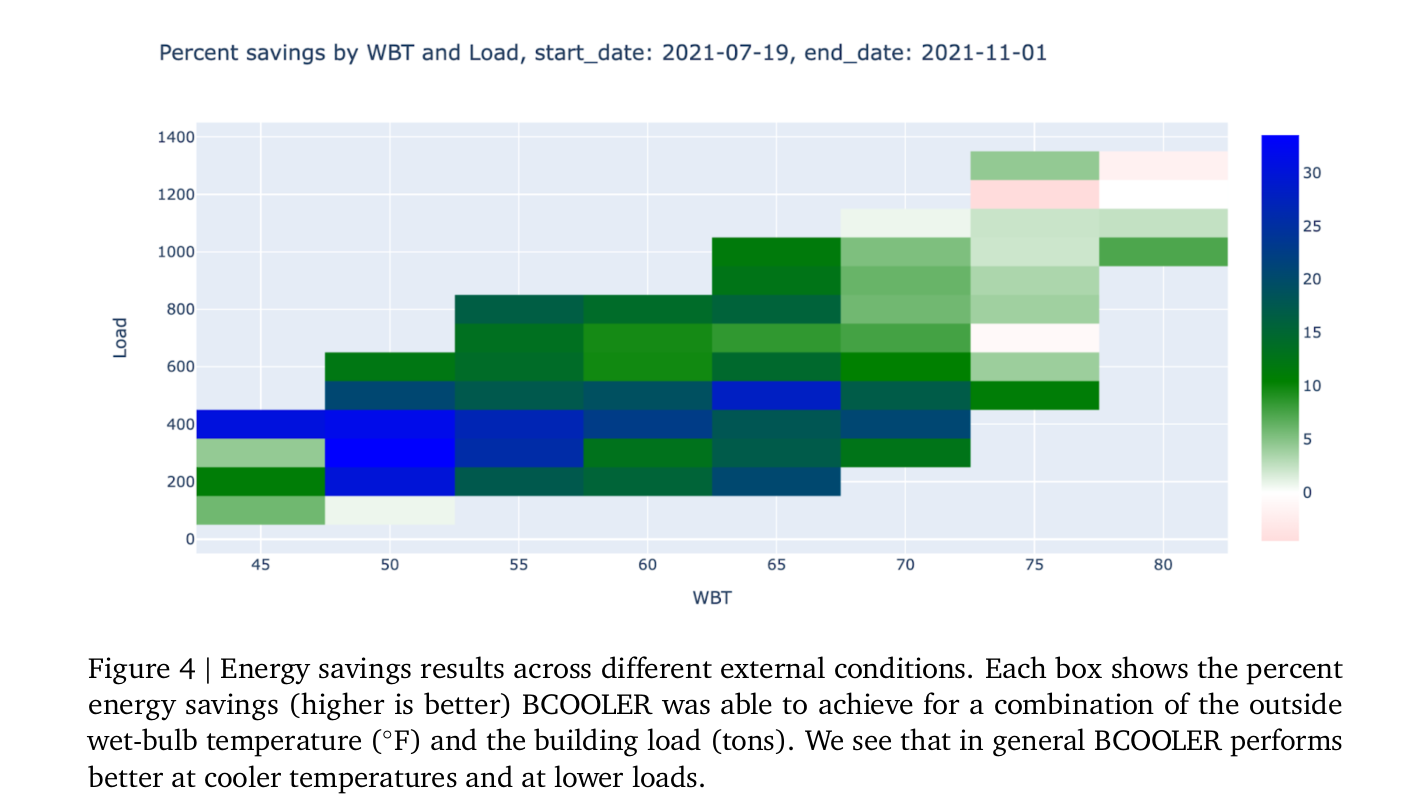
\includegraphics[width=3in]{Screenshot from 2023-05-20 22-20-56.png}
    \caption{The method by which Deepmind compared the performance of BCOOLER against the original SOO \cite{luo2022controlling}. The method compares average energy-to-load efficiencies for comparable loads and WBTs. The loads and WBTs account for the difficulty the algorithms have to find an energy-efficient action.}
    \label{fig:my_label}
\end{figure}

This method of comparison seems to regularize for most confounders because it stratifies the sample for various loads. It has proved itself in the aforementioned research. We will use this as the method of benchmarking $A$ against the original SOO, both for simulation measurements as for measurements obtained in the live trials. The only think we need to do is to find the appropriate literature on stratified statistical testing in order to turn this visual approach into a quantitative statistical test. We can try various numbers of partitions along the WBT and along the estimated load, and perform univariate $t$-tests per partition. There is a catch to this, namely that when performing many univariate tests, the $p$-value has to be discounted, see chap. 4 of \cite{091a7cc2b3e34c708e1bedf1387c10c1}. So even though we collect data from very many time points (every 5 minutes for a year), the partition cannot be too fine.

\subsubsection{Triangulation}
We use two independent methods of data collection, namely via simulation and via an on-site experiment. The two complement each other in the following way: on the one hand, simulation can generate much more data at a much lower cost to achieve statistically significant results within a reasonable budget. On the other hand, on-site testing is necessary to verify that the model also performs under real physical conditions. If the results are comparable enough, this will reinforce the results from the simulation.

Another data generation method is a survey of the satisfaction of building occupants, which is also an ethical measure to ensure their comfort. This survey will be discussed in detail under \ref{Ethical considerations}

\subsection{Ethical considerations} \label{Ethical considerations}
\subsubsection{Enforcing safety using hierarchical controller and hard constraints on buildin temperatures}
In terms of ethics, we need to take into account the comfort of building occupants. The function $J$ includes penalty terms enforcing soft constraints that require the agent to maintain temperatures within a reasonable distance from the setpoint.

We do however not want to take the risk of the RL agent ``misbehaving'' because these penalty terms are not strong enough. We enforce this as follows:
\begin{enumerate}
    \item State hard constraints to keep track of: in particular, ensure that the bounds around the thermostat temperature setpoints are tight enough. An initial bound of around 1.5 degrees Celsius might be reasonable.
    \item Only proceed to live testing when the RL agent does not violate these constraint during simulation in the simulated building environment.
    \item If the constraint is violated during life testing, let the original SOO take over control of the system: this is the so-called hierarchical approach.
\end{enumerate}

The only problem that might arise is that the algorithm acts biased towards certain zones or rooms of the building, in the sense that maintaining the setpoint temperature in this wing will comes at higher power consumption increase than in the other wing, so the algorithm will systematically stay closer to the demanded setpoints in the other wing. An example would be that during summer, the side of the building that receives direct sunlight is kept at a warmer temperature than the shadow side as the efficiency of airconditioning.

If such problems do arise, we need to provide building occupants with a way to anonymously speak up about this. Complaints should be collected via regularly posted, anonymized surveys which are distributed via a mailing list. This survey should ask: 
\begin{enumerate}
    \item whether there are complaints with regards to the HVAC in the office, and what the nature of this complaint is (i.e. too hot, too cold, too much noise).
    \item a clickable floor plan of the building in which one or more of the aforementioned segments can be selected as being the place of the complaint.
    \item a blank field into which the participant can write any questions with regards to the experiment. These questions must be linked to an email address for the sake of answering them but they are not linked to the preceding questions.
\end{enumerate}

The possibility of asking questions is important to maintain transparency about the research towards the occupants of the building. They are, after all, participants in an experiment so it would be ethical to be open about the nature of the experiment.

\subsection{Legal considerations}
\subsubsection{Implicit consent of building occupants}
Finally, since the building occupants are in a sense involuntarily involved with an experiment, we should look into the legal details of this. In particular, is the consent of the building tenant enough to run the experiment? This depends on the contract between the offices and the building tenant.

\subsubsection{Intellectual property}
Our model $A$ might be trained in a simulated building environment that was designed by the engineering company for Mercator II. We need to take into account that we reuse a considerable part of their design, upon which some licensing might rest. If this licensing does not allow the reuse of the design for experimental purposes, we need to redesign our own physical model of the environment. We then proceed as under \ref{Method:setup}.

\subsection{Time plan} \label{time plan}
\FloatBarrier
Here we discuss the planning for each part of the design and creation of model $A$ and $B$ and the schedule for simulation and live-testing of different model architectures against the original SOO:

\begin{table}
\centering\begin{tabular}{r|p{5in}}

Month & Activity\\ 
\hline
1,2 & Consult Radboud University and Boonstoppel (now Deerns) for design plans and simulation environment of Mercator II. Inventarize the available sensors, thermostats and actuators at the facility. Get access to the building simulation of the engineers. Collect historical data from the system. Investigate the provided variables and their units of measure. Ask about the choice of variables by the engineer, reformulate a the state variables if adviced by the engineering team. Import the MPC that will be used for $B$ from another building. \\
\hline
3,4,5 & \textit{Risk:} no acces to simulation model. In this case, we have to import $B$ from \cite{hollands} and train its parameters on historical data of Mercator II, and later design a simulation model in HVACSIM+ for evaluation of the agent. This needs another 3 months of design and literature research into built environment models.\\
\hline
6,7 & Literature research into model-based RL and MPC. Investigate the choices for importable MPC models for $B$. Especially, how does the optimization over a finite horizon in the MPC work in practice? Model-based reinforcement learning and model-predictive control are closely related and often only different in terminology, see i.e. \cite{Seita_2019}. Publish a temporary proceedings paper regarding the unification of terminology of RL and MPC.\\
\hline
7, 8 & Literature research into the evaluation of efficiency of HVAC control models. Is the approach taken by \cite{luo2022controlling} indeed statistically sound, and where to find the details? Formulate our own test statistic and prepare means by which to visualize the performance measurement data.\\
\hline
9,10 & Formulate a suitable model architecture $C$. These can be based on BCOOLER's architecture for value-function approximation (utilizes convolutional layers) since that architecture has proven itself in previous research \cite{luo2022controlling}. The cost function and MPC model are imported and thus need not be formulated.\\
\hline
11,12 & Research into software frameworks to build RL agents in (not covered in this proposal). Look into how it is most efficient to integrate an MPC into the agent. Import a suitable framework and test it. Second month, look into frameworks for neural networks that model $C$ can be programmed in.\\
\hline
11,12 & Programming and Simulation of various predictors $C$. Also simulate the original SOO of Mercator II and see if there is an improvement for some of the models. Select these models for live testing \\
\hline
13-24 & Live testing of $A$ at the facility (1 year period, interrupted if complaints or issues are raised). One year is strictly necessary to account for change of seasons, see e.g. \cite{luo2022controlling}. We do not need another year to test the original SOO since we can use its historical power consumption data as measurements.\\
\hline
26, 27 & Data analysis: employ the statistical method developed in week 7, 8 to evaluate the performance increase/decrease of the model. Draw a conclusion. \\
\hline
28 & Compose the paper reporting on the conclusion. If negative, put emphasis on the new framework $A$ is based on and propose the usage of a different internal MPC $B$ or a different action-value predictor $C$.\\
\hline
29 & Publish the code used in the research. For the ultimate benefit of the environment and science, we decide upon open-sourcing the designed software framework for future research to use.\\

\end{tabular}
\caption{The timeline for the proposed research.}
\end{table}

The aim is to complete the research within 2 years and 6 months. If a simulation model in a building energy simulator for Mercator II is available, this reduces the total time by 3 months. If an MPC controller for Mercator II is available, another 3 months are deducted. The estimates of three months for the design and parameter estimation of an MPC is quite pessimistic; we might be able to save some time here.


\begin{multicols}{2}
    
\bibliographystyle{plain}
\bibliography{references.bib}
\end{multicols}

\end{document}